%!TEX root = ../main.tex
\begin{frame}{Tarefa de Aprendizado}
\begin{itemize}
  \item \alert{Tarefa de Regressão}
  \item \alert{Entrada}:
  \begin{itemize}
    \item Imagem em cores RGB de dimensões $224 \times 224$ pixels contendo uma face humana centralizada
  \end{itemize}
   \item \alert{Saída}:
   \begin{itemize}
        \item Estimativa de idade, em anos, da pessoa correspondente
   \end{itemize}
\end{itemize}
\begin{center}
     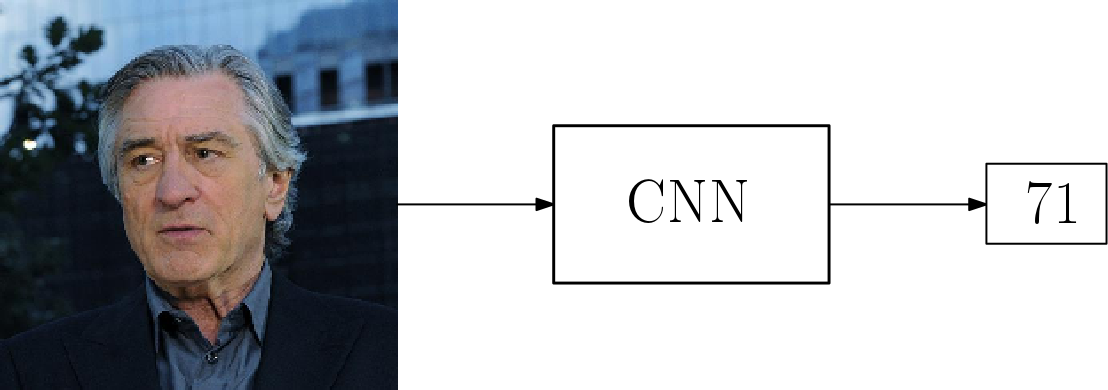
\includegraphics[width=0.60\textwidth]{img/deniro_cnn}
\end{center}
\end{frame}

\begin{frame}{Tarefa de Aprendizado}
     \begin{itemize}
          \item Métricas de desempenho:
          \begin{itemize}
            \item \emph{Root Mean Squared Error} (RMSE)
     \begin{equation}\label{eq:rmse}
          \textrm{RMSE} = \sqrt{\frac{1}{n} \sum_{i=1}^n (y_i - \hat{y})^2}.
     \end{equation}
           \item \emph{Mean Absolute Error} (MAE)
         \end{itemize}
    \end{itemize}
    \begin{equation}\label{eq:mae}
         \textrm{MAE} = \frac{1}{n}\sum_{i=1}^{n} |y_i - \hat{y}|
    \end{equation}
  \end{frame}

\begin{frame}{Conjunto de Dados}
  \begin{itemize}
    \item Base de dados experimentais IMDb
    \begin{itemize}
      \item $452.132$ exemplos
      \item $20.284$ dos atores mais populares listados no site IMDb
      \item Organizada por Rothe et al., 2015
      \item Imagens e meta-dados
    \end{itemize}
  \end{itemize}
\end{frame}

\begin{frame}{Conjunto de Dados}
     \ \  \\[0.1cm]
     \begin{figure}[ht]
          \label{tab:um_deniro}
               \begin{minipage}[c]{0.62\linewidth}
               \begin{small}
               \centering
               \begin{tabular}{p{3.3cm} p{5cm}}\toprule
                    \textbf{Meta-dado} & \textbf{Valor} \\ \midrule
                    ID Celebridade & 16349 \\
                    Nome & Robert De Niro \\
                    Endereço da imagem & \footnotesize{imdb$/$34$/$nm0000134$\_$rm334009 0368$\_$1943-8-17$\_$2011.jpg} \\
                    Pontuação da Face & $5.21396$ \\
                    Pontuação da Segunda Face & NaN \\
                    Localização da Face & $(663.65, 992.475, $ $590.134, 918.959)$ \\
                    Data de Nascimento  & $1943-08-17$\\
                    Ano da Foto & 2011 \\
                    Gênero & Masculino \\
                    \bottomrule
               \end{tabular}
          \end{small}
          \end{minipage}
          \hfill
          \begin{minipage}[c]{0.3\linewidth}
               \centering
               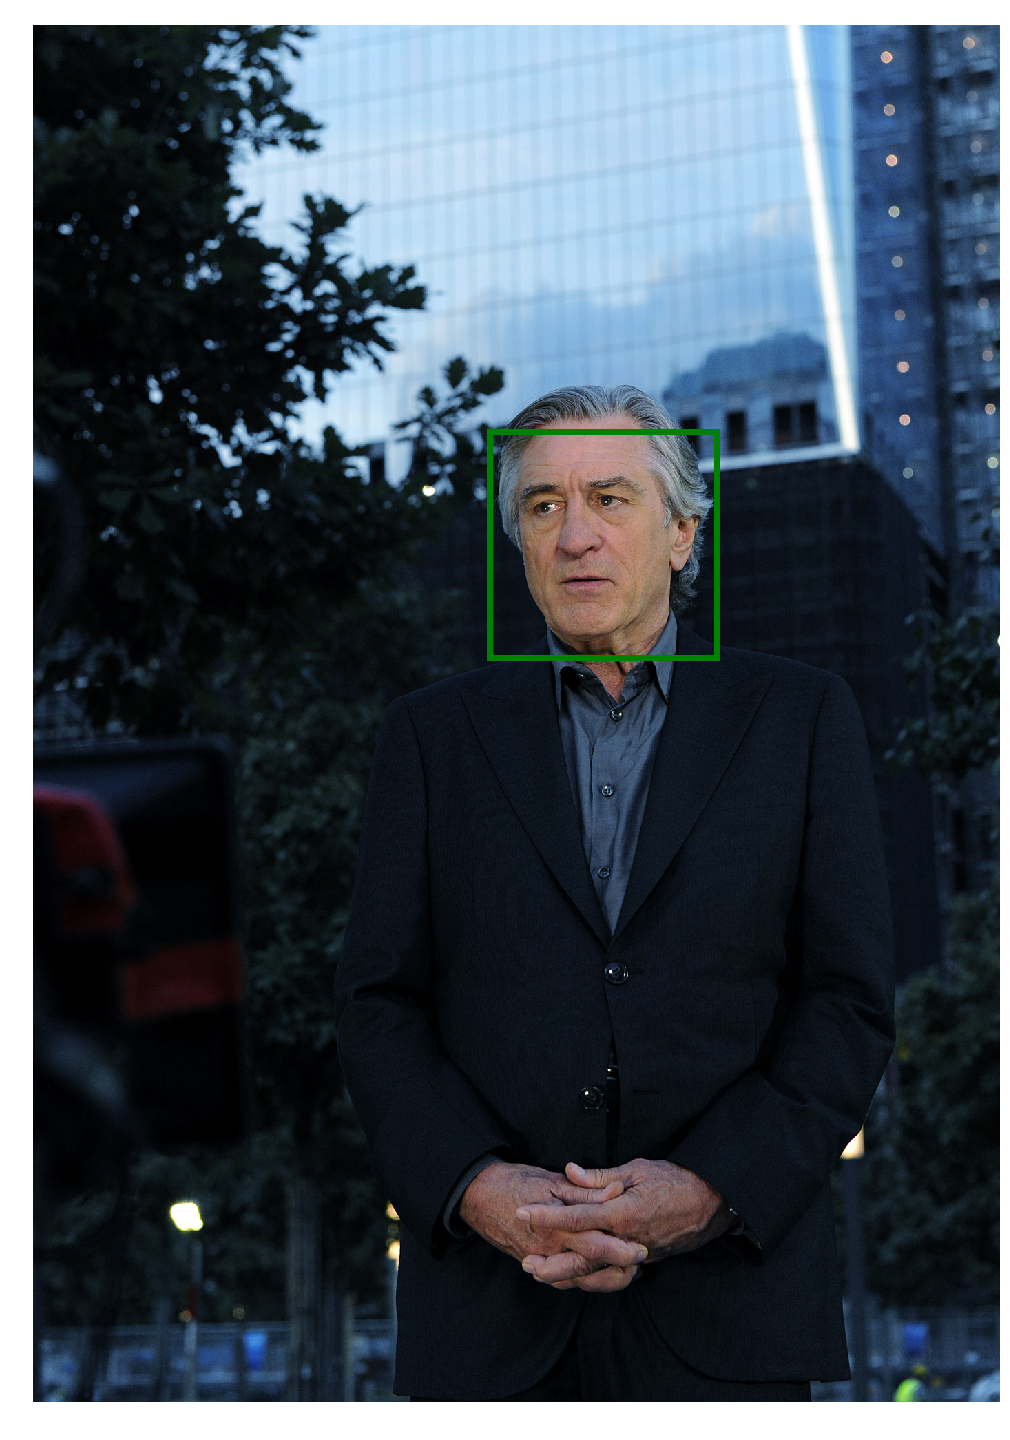
\includegraphics[width=\linewidth]{img/deniro_plt}
          \end{minipage}
          \caption{Exemplo de imagem do conjunto de dados contendo apenas um rosto.}
     \end{figure}
\end{frame}

\begin{frame}{Conjunto de Dados}
     \ \  \\[0.1cm]
     \begin{figure}[ht]
          \label{tab:dois_deniro_errado}
               \begin{minipage}[c]{0.62\linewidth}
               \begin{small}
               \centering
               \begin{tabular}{p{3.3cm} p{5cm}}\toprule
                    \textbf{Meta-dado} & \textbf{Valor} \\ \midrule
                    ID Celebridade & 16349 \\
                    Nome & Robert De Niro \\
                    Endereço da imagem & \footnotesize{imdb$/$34$/$nm0000134$\_$rm14800 44288$\_$1943-8-17$\_$2012.jpg} \\
                    Pontuação da Face & $5.51656$ \\
                    Pontuação da Segunda Face & $4.55379$ \\
                    Localização da Face & $(1392.72, 1614.18, $ $225.55, 447.003)$ \\
                    Data de Nascimento  & $1943-08-17$\\
                    Ano da Foto & 2012 \\
                    Gênero & Masculino \\ \bottomrule
               \end{tabular}
          \end{small}
          \end{minipage}
          \hfill
          \begin{minipage}[c]{0.35\linewidth}
               \centering
               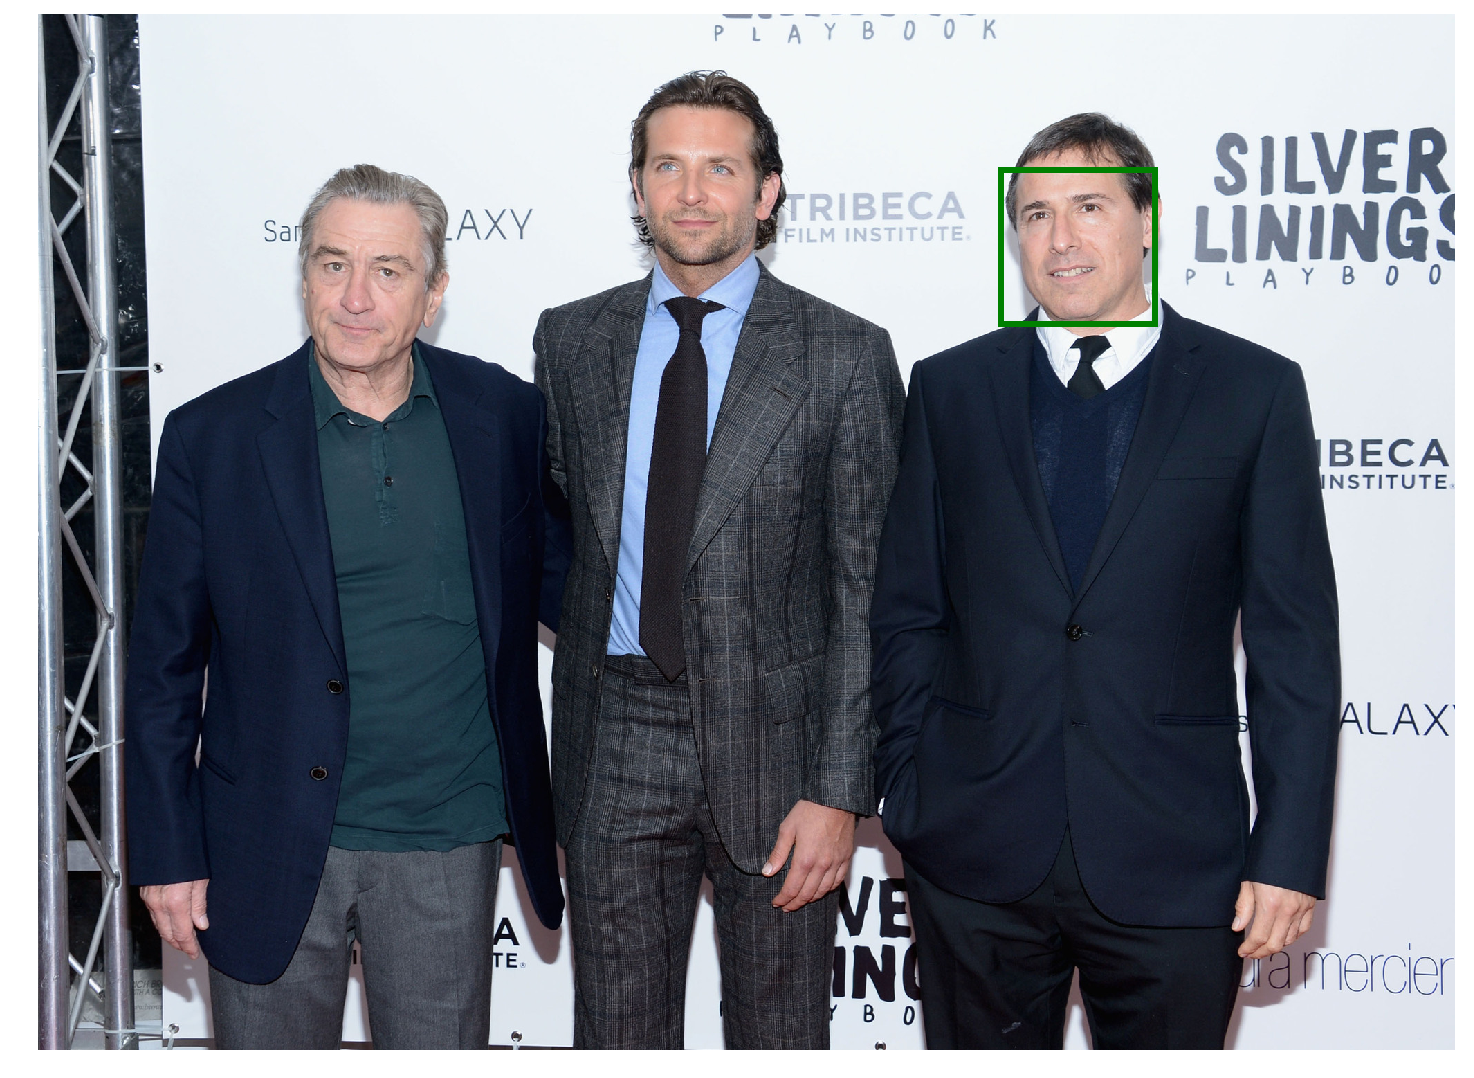
\includegraphics[width=\linewidth]{img/deniro_many_plt_errado}
          \end{minipage}
          \caption{Exemplo de imagem do conjunto de dados contendo mais de um rosto com a classificação errônea.}
     \end{figure}
\end{frame}

\begin{frame}{Limpeza e Pré-processamento dos dados}
     \begin{itemize}
       \item Versão original: $267$ GB
       \item Faces recortadas: $7,1$ GB
       \ \ \newline
          \item Cálculo do atributo alvo: \alert{Idade}
          \ \ \newline
          \item Itens descartados:
          \begin{itemize}
               \item Idade e gênero apresentando valores nulos, inválidos ou negativos
               \item Múltiplos exemplos referentes à mesma pessoa com a mesma idade
               \item Idade maior que $100$ anos ou não compatível com os dados da celebridade referida nos meta-dados
               \item Ausência de rosto
               \item Presença de mais de uma face na imagem
          \end{itemize}
     \end{itemize}
\end{frame}

\begin{frame}{Limpeza e Pré-processamento dos dados}
     \begin{itemize}
          \item Padronização das dimensões das imagens
          \begin{itemize}
               \item $224 \times 224$ \emph{pixels}
               \item RGB
          \end{itemize}
          \  \ \newline
          \item Descarte de meta-dados irrelevantes para a tarefa de aprendizado
     \end{itemize}
\end{frame}

\begin{frame}{Limpeza e Pré-processamento dos dados}
     \begin{itemize}
          \item Equalização por histograma
          \begin{figure}[!ht]
          	%\caption{Exemplo de imagem do conjunto de dados antes e depois do processo de equalização por histograma.}
          	%\label{fig:equalizacao}
          	\centering
          	\begin{subfigure}[h]{0.4\linewidth}
          		\caption{Imagem sem equalização de histograma.}
          		\label{fig:eq_antes}
          		\centering
          		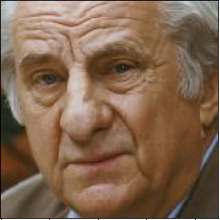
\includegraphics[width=0.8\linewidth]{img/solucao/hist_eq_orig.png}
          	\end{subfigure}
          	\hspace{0.1cm}
          	\begin{subfigure}[h]{0.4\linewidth}
          		\caption{Imagem após equalização por histograma.}
          		\label{fig:eq_depois}
          		\centering
          		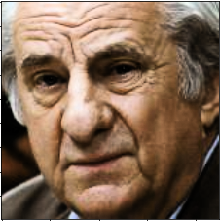
\includegraphics[width=0.8\linewidth]{img/solucao/hist_eq_mod.png}
          	\end{subfigure}
          \end{figure}
     \end{itemize}
\end{frame}

\begin{frame}{Limpeza e Pré-processamento dos dados}
     \begin{itemize}
          \item Conjunto de dados consolidado:
          \begin{itemize}
               \item $47.950$ exemplos
               \item $14.607$ celebridades
               \item $1,2 GB$ em disco
          \end{itemize}
          \ \ \newline
          \item Divisão obedecendo o método \emph{Holdout}
          \begin{itemize}
               \item Treinamento$-$Validação$-$Teste
               \item $70\%-10\%-20\%$
               \item $33.565-4.795-9.590$
          \end{itemize}
     \end{itemize}
\end{frame}

\begin{frame}{Modelos de CNN Considerados}
     \begin{itemize}
          \item Arquiteturas
          \begin{itemize}
            \item LeNet
            \item AlexNet
            \item VGG-16
            \item SqueezeNet
          \end{itemize}
     \end{itemize}
\end{frame}

\begin{frame}{Modelos de CNN Considerados}
     \begin{itemize}
          \item Funções de ativação: \emph{ReLU} ou \emph{Leaky ReLU}
          \item Método de otimização do gradiente descendente \emph{Adam}
          \item Taxa de aprendizado de $0.001$
          \ \ \newline
          \item Camadas de saída com apenas um neurônio
          \item \emph{batch size} igual a $64$
          \item Número de épocas obtido de maneira experimental
     \end{itemize}
\end{frame}
